\documentclass[12pt]{article}

\usepackage[utf8]{inputenc}
\usepackage[T1, T2A]{fontenc}
\usepackage[russian]{babel}

\usepackage{amsmath,amssymb}

\usepackage{float}
\usepackage{graphicx}
\graphicspath{ {./pic/} }

\title{Байесовская деконволюция для эксперимента СФЕРА-2}

\author{Игорь Вайман}

\date{\today}

\begin{document}
	\maketitle
	
	\section{Описание эксперимента}

	Эксперимент СФЕРА-2 основан на сборе и регистрации черенковского света ШАЛ, отражённого от <<экрана>> -- ровной заснеженной поверхности льда озера Байкал. Установка представляет собой сферическое зеркало и мозаику ФЭУ, установленную вблизи фокальной поверхности. Черенковский свет ШАЛ, рассеиваясь на снегу, проходит через диафрагму установки, отражается от зеркала, и попадает на фотокатод. При попадании фотона с длиной волны в области чувствительности фотокатода с него выбиваются $1 - 10$ (уточнить) вторичных электронов, которые проходят систему динодов с разностью потенциалов между каждой парой, создавая в результате избыточный на аноде. Этот заряд стекает с анода через цепь усиления, создавая в результате напряжение на входе АЦП. Это напряжение считывается электроникой, в результате и составляя (вместе с некоторой телеметрией) экспериментальные данные.
	
	Этот набор физических процессов мы описываем в следующих предположениях:
	
	\begin{enumerate}
		\item В системе нет электронных шумов -- единственным источником шума являются фоновые фотоны (от звёздного и зодиакального света, так как эксперимент проводится в ясные безлунные ночи). Фотоны шума попадают в установку аналогично <<сигнальным>> фотонам -- после рассеяния на поверхности. Их поток можно приблизительно оценить по каталогам светимости звёзд и из моделей зодиакального света. (Ссылка на работу Энтиной)
		\item Работу ФЭУ можно эффективно описать одной <<рандомизированной>> испульсной характеристикой (РИХ). Понятие и применение РИХ будет раскрыто далее, в общем виде это случайная функция времени, описывающая отклик системы на один фотон, падающий на фотокатод. Главный источник случайности в установке СФЕРА-2 -- неопределённость числа вторичных фотонов, вылетевших с фотокатода, приводящая к неопределённости амплитуды импульса тока. Стоит отметить, что случайный характер ИХ проявляется именно на границе между режимом счёта фотонов и режимом измерения потока, поскольку поток фотонов уже слишком велик, чтобы разрешать отдельные импульсы, но недостаточно -- чтобы случайные характеристики эффективно усреднялись. Мы также предполагаем, что случайность импульсной характеристики проявлялась независимо между отдельными фотонами и между разными ФЭУ.
		\item Используя экспериментальные данные (данные, записанные АЦП, постоянную компоненту анодного тока и абсолютную калибровку ФЭУ) мы можем восстановить показания анодного тока (ссылка на работу по электронике). Неопределённость, вносимая анодной цепью, усилителем и (главным образом) дискретизацией сигнала на входе АЦП, хорошо известна и учитывается во вторую очередь.
	\end{enumerate}

	\section{Постановка задачи}
	
	\subsection{Упрощённая модель}
	
	Рассмотрим $N$ последовательных равновеликих временных бинов. Для простоты будем считать единицей времени длительность одного бина. Тогда мы можем задать временные бины интервалами $[i-1, i]$, $i = 1 \ldots N$. Обозначим число фотонов в каждом бине как $n_i$, $i = 1, \ldots, N$.
	
	Распределение времён прихода фотонов внутри одного бина, вообще говоря, может быть произвольным, однако в простейшей модели можно считать его равномерным. Это оправдано для независимых друг от друга фоновых фотонов, и может служить приближением для фотонов ШАЛ в случае, если дисперсия времён прихода фотонов внутри <<пакета>> сильно превышает длительность временного бина. По данным модельных ливней это не всегда так, поэтому влияние неравномерности распределения времён прихода фотонов будет исследовано отдельно.
	
	Далее положим, что импульсная характеристика является конечной во времени и длится не более чем $L$ временных бинов. Тогда сигнал на выходе системы полностью содержится в интервале $[0, N + L]$, так как самое позднее время прихода фотона -- правая граница последнего бина.
	
	Будем считать, что АЦП записывает значения сигнала $S_j$ в точках $j = 0, 1, \ldots, N + L$. Впрочем, $S_0 = 0$ с вероятностью $1$, поэтому можно исключить его из рассмотрения.
	
	Поставим задачу <<байесовской деконволюции>> следующим образом, используя байесовскую терминологию: зная рандомизированную импульсную характеристику системы и значения $S_j, \; j = 1, \ldots, N + L$, оценить апостериорные функции плотности вероятности для значений $n_i$, $i = 1, \ldots, N$. В качестве априорного распределения $n_i$ используется наивное неограниченное однородное распределение ($p_{n_i}(x) = Const \; \forall x \in [0, \infty)$).
	
	Заметим, что, в отличие от обычной деконволюции, мы не ставим задачу оценить исходный сигнал -- в данном случае представляющий собой сумму $\delta$-функций с соответствующими сдвигами -- но только его аггрегированную характеристику. Информация об отдельных фотонах не является необходимой для обработки экспериментальных событий, и её получение представляет собой, по-видимому, более трудную задачу.
	
	Легко заметить также, что в реальном эксперименте мы имеем дело с неограниченным во времени потоком фотонов, а не с изолированными $N$ бинами -- эффекты на краях области регистрации сигнала нужно будет учитывать отдельно.
	
	Иллюстрация постановки задачи приведена на рис. \ref{pic:problem-setup}.
	
	\begin{figure}[H]
		\centering
		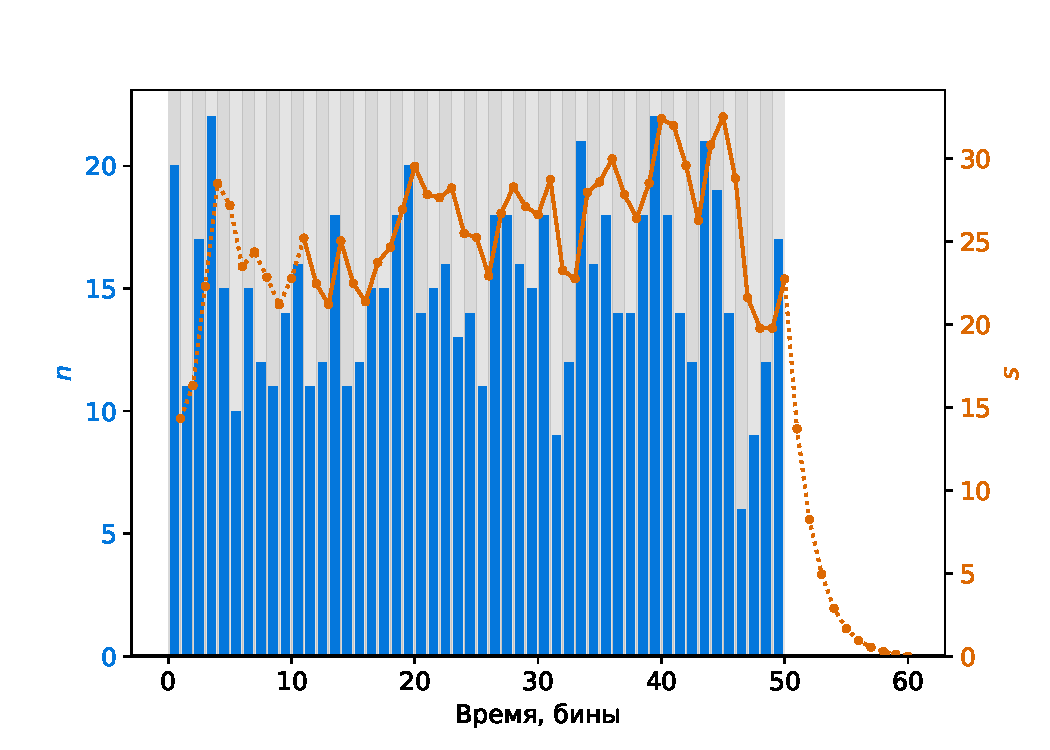
\includegraphics[width=\columnwidth]{problem-setup-example}
		\caption{Пример данных для задачи байесовской деконволюции. Здесь $N = 50$, количество фотонов в каждом бине определено из пуассоновского распределения с $\lambda = \mathbb{E}(n_i) = 15$; РИХ для простоты положена детерминистичной функцией $\exp(-t)$ с $L = 10$. Задача состоит в том, чтобы, зная значения выходного сигнала (оранжевый) и РИХ, оценить апостериорные распределения количества фотонов в каждом бине (синих столбцов).}
		\label{pic:problem-setup}
	\end{figure}
	
\end{document}
